\documentclass{standalone}
\usepackage{tikz}
\usepackage{calc}
\usepackage{pgffor}
\usetikzlibrary{patterns}
\begin{document}
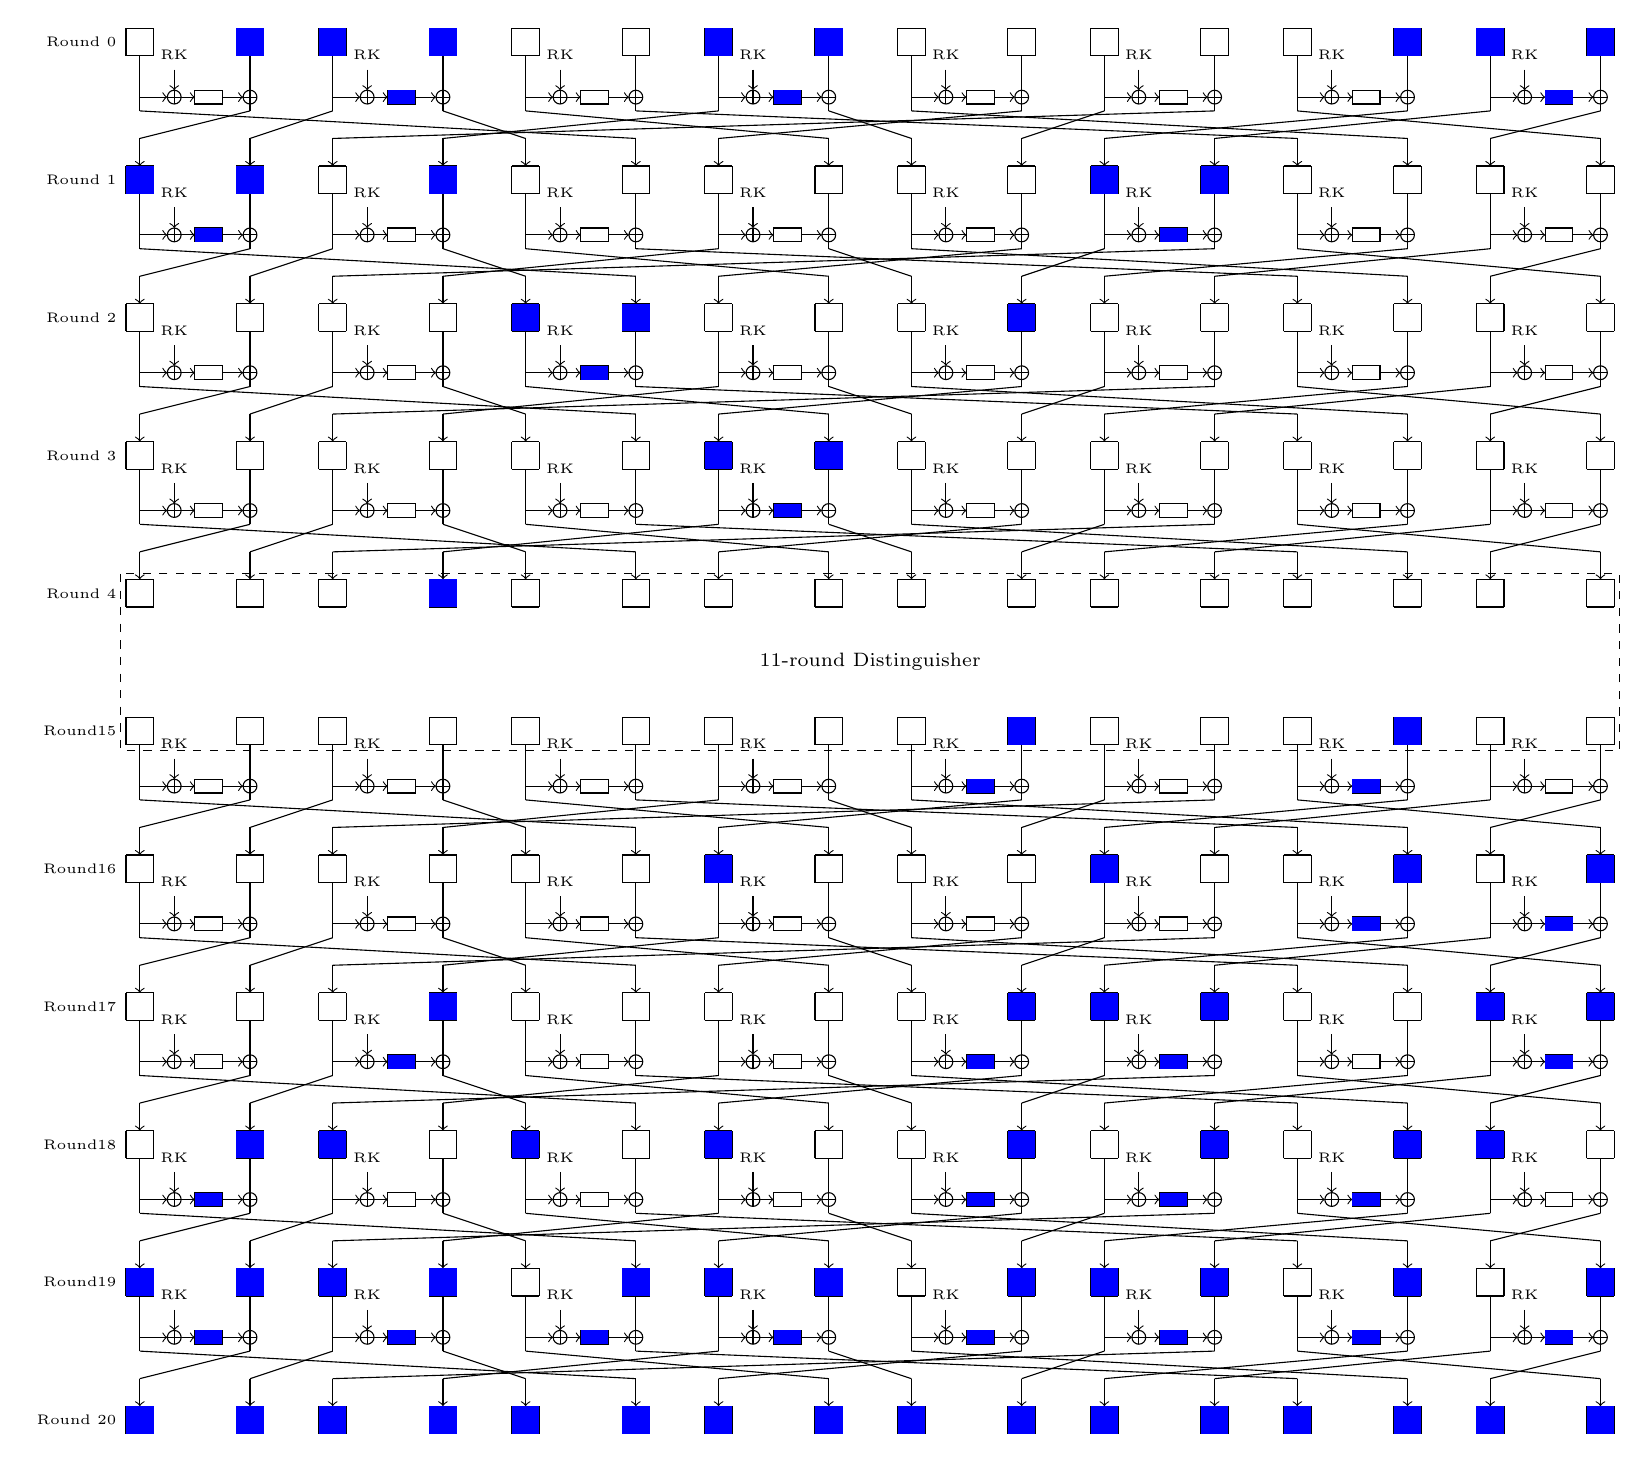
\begin{tikzpicture}[scale=0.35]
\foreach \z in {0,1,2,3}{
\begin{scope}[yshift = -\z* 5 cm]
\node[left] at (0,0.5) {\tiny Round \z};
\foreach \x  in {0,1,...,7}
{
\begin{scope}[xshift = \x*7 cm]
\draw (0,0) grid +(1,1);
\draw[->] (0.5,0)|- +(1,-1.5);
\draw (4,0) grid +(1,1);
\draw (1.75,-1.5) circle (0.25);
\draw (1.75,-1.25) --+(0,-0.5);
\draw[->] (1.5,-1.5) --(2.5,-1.5);
\draw (2.5,-1.75) rectangle + (1,0.5);
\draw[->](3.5,-1.5)--(4.25,-1.5);
\draw (4.5,-1.5) circle (0.25);
\draw (4.25,-1.5) -- +(0.5,0);
\draw (4.5,0)--+(0,-2);
\draw[->](0.5,-3)--+(0,-1);
\draw[->](4.5,-3)--+(0,-1);
\draw (0.5,-1.5)--+(0,-0.5);
\draw[->] (1.75,-0.5) node[above]{\tiny{RK}} --(1.75,-1.25);
\end{scope}

}
\end{scope}
}

\foreach \z in {0,1,2,3}{
\begin{scope}[yshift = -\z* 5 cm]
\draw (0.5,-2)--(18.5,-3);
\draw (4.5,-2)--(0.5,-3);
\draw (7.5,-2)--(4.5,-3);
\draw (11.5,-2)--(14.5,-3);
\draw (14.5,-2)--(25.5,-3);
\draw (18.5,-2)--(42.5,-3);
\draw (21.5,-2)--(11.5,-3);
\draw (25.5,-2)--(28.5,-3);
\draw (28.5,-2)--(46.5,-3);
\draw (32.5,-2)--(21.5,-3);
\draw (35.5,-2)--(32.5,-3);
\draw (39.5,-2)--(7.5,-3);
\draw (42.5,-2)--(53.5,-3);
\draw (46.5,-2)--(35.5,-3);
\draw (49.5,-2)--(39.5,-3);
\draw (53.5,-2)--(49.5,-3);
\end{scope}
}

\begin{scope}[yshift = -20cm]
\foreach \x  in {0,1,...,7}
{
\begin{scope}[xshift = \x*7 cm]
\draw (0,0) grid +(1,1);
\draw (4,0) grid +(1,1);
\end{scope}
}

\node[left] at (0,0.5) {\tiny Round 4};
\end{scope}
\begin{scope}[yshift = -20cm]
\draw[dashed] (-0.2,1.2) rectangle node{\scriptsize 11-round Distinguisher} +(54.4,-6.4);
\end{scope}

\foreach \z in {5,6,7,8,9}{
\begin{scope}[yshift = -\z* 5 cm]
\node[left] at (0,0.5) {\tiny Round\pgfmathparse{int((\z-1)+11)}\pgfmathresult};
\foreach \x  in {0,1,...,7}
{
\begin{scope}[xshift = \x*7 cm]
\draw (0,0) grid +(1,1);
\draw[->] (0.5,0)|- +(1,-1.5);
\draw (4,0) grid +(1,1);
\draw (1.75,-1.5) circle (0.25);
\draw (1.75,-1.25) --+(0,-0.5);
\draw[->] (1.5,-1.5) --(2.5,-1.5);
\draw (2.5,-1.75) rectangle + (1,0.5);
\draw[->](3.5,-1.5)--(4.25,-1.5);
\draw (4.5,-1.5) circle (0.25);
\draw (4.25,-1.5) -- +(0.5,0);
\draw (4.5,0)--+(0,-2);
\draw[->](0.5,-3)--+(0,-1);
\draw[->](4.5,-3)--+(0,-1);
\draw (0.5,-1.5)--+(0,-0.5);
\draw[->] (1.75,-0.5) node[above]{\tiny{RK}} --(1.75,-1.25);
\end{scope}

}
\end{scope}
}

\foreach \z in {5,6,7,8,9}{
\begin{scope}[yshift = -\z* 5 cm]
\draw (0.5,-2)--(18.5,-3);
\draw (4.5,-2)--(0.5,-3);
\draw (7.5,-2)--(4.5,-3);
\draw (11.5,-2)--(14.5,-3);
\draw (14.5,-2)--(25.5,-3);
\draw (18.5,-2)--(42.5,-3);
\draw (21.5,-2)--(11.5,-3);
\draw (25.5,-2)--(28.5,-3);
\draw (28.5,-2)--(46.5,-3);
\draw (32.5,-2)--(21.5,-3);
\draw (35.5,-2)--(32.5,-3);
\draw (39.5,-2)--(7.5,-3);
\draw (42.5,-2)--(53.5,-3);
\draw (46.5,-2)--(35.5,-3);
\draw (49.5,-2)--(39.5,-3);
\draw (53.5,-2)--(49.5,-3);
\end{scope}
}

\begin{scope}[yshift = -50cm]
\foreach \x  in {0,1,...,7}
{
\begin{scope}[ xshift = \x*7 cm]
\draw (0,0) grid +(1,1);
\draw (4,0) grid +(1,1);
\end{scope}
}

\node[left] at (0,0.5) {\tiny Round 20};
\end{scope}
\begin{scope}[yshift = -0cm]
\fill[blue] (9.5,-1.75) rectangle+(1,0.5);
\fill[blue] (23.5,-1.75) rectangle+(1,0.5);
\fill[blue] (51.5,-1.75) rectangle+(1,0.5);
\fill[blue] (4,0) rectangle+(1,1);
\fill[blue] (7,0) rectangle+(1,1);
\fill[blue] (11,0) rectangle+(1,1);
\fill[blue] (21,0) rectangle+(1,1);
\fill[blue] (25,0) rectangle+(1,1);
\fill[blue] (46,0) rectangle+(1,1);
\fill[blue] (49,0) rectangle+(1,1);
\fill[blue] (53,0) rectangle+(1,1);
\end{scope}

\begin{scope}[yshift = -5cm]
\fill[blue] (2.5,-1.75) rectangle+(1,0.5);
\fill[blue] (37.5,-1.75) rectangle+(1,0.5);
\fill[blue] (0,0) rectangle+(1,1);
\fill[blue] (4,0) rectangle+(1,1);
\fill[blue] (11,0) rectangle+(1,1);
\fill[blue] (35,0) rectangle+(1,1);
\fill[blue] (39,0) rectangle+(1,1);
\end{scope}

\begin{scope}[yshift = -10cm]
\fill[blue] (16.5,-1.75) rectangle+(1,0.5);
\fill[blue] (14,0) rectangle+(1,1);
\fill[blue] (18,0) rectangle+(1,1);
\fill[blue] (32,0) rectangle+(1,1);
\end{scope}

\begin{scope}[yshift = -15cm]
\fill[blue] (23.5,-1.75) rectangle+(1,0.5);
\fill[blue] (21,0) rectangle+(1,1);
\fill[blue] (25,0) rectangle+(1,1);
\end{scope}

\begin{scope}[yshift = -20cm]
\fill[blue] (11,0) rectangle+(1,1);
\end{scope}

\begin{scope}[yshift = -25cm]
\fill[blue] (30.5,-1.75) rectangle+(1,0.5);
\fill[blue] (44.5,-1.75) rectangle+(1,0.5);
\fill[blue] (32,0) rectangle+(1,1);
\fill[blue] (46,0) rectangle+(1,1);
\end{scope}

\begin{scope}[yshift = -30cm]
\fill[blue] (44.5,-1.75) rectangle+(1,0.5);
\fill[blue] (51.5,-1.75) rectangle+(1,0.5);
\fill[blue] (21,0) rectangle+(1,1);
\fill[blue] (35,0) rectangle+(1,1);
\fill[blue] (46,0) rectangle+(1,1);
\fill[blue] (53,0) rectangle+(1,1);
\end{scope}

\begin{scope}[yshift = -35cm]
\fill[blue] (9.5,-1.75) rectangle+(1,0.5);
\fill[blue] (30.5,-1.75) rectangle+(1,0.5);
\fill[blue] (37.5,-1.75) rectangle+(1,0.5);
\fill[blue] (51.5,-1.75) rectangle+(1,0.5);
\fill[blue] (11,0) rectangle+(1,1);
\fill[blue] (32,0) rectangle+(1,1);
\fill[blue] (35,0) rectangle+(1,1);
\fill[blue] (39,0) rectangle+(1,1);
\fill[blue] (49,0) rectangle+(1,1);
\fill[blue] (53,0) rectangle+(1,1);
\end{scope}

\begin{scope}[yshift = -40cm]
\fill[blue] (2.5,-1.75) rectangle+(1,0.5);
\fill[blue] (30.5,-1.75) rectangle+(1,0.5);
\fill[blue] (37.5,-1.75) rectangle+(1,0.5);
\fill[blue] (44.5,-1.75) rectangle+(1,0.5);
\fill[blue] (4,0) rectangle+(1,1);
\fill[blue] (7,0) rectangle+(1,1);
\fill[blue] (14,0) rectangle+(1,1);
\fill[blue] (21,0) rectangle+(1,1);
\fill[blue] (32,0) rectangle+(1,1);
\fill[blue] (39,0) rectangle+(1,1);
\fill[blue] (46,0) rectangle+(1,1);
\fill[blue] (49,0) rectangle+(1,1);
\end{scope}

\begin{scope}[yshift = -45cm]
\fill[blue] (2.5,-1.75) rectangle+(1,0.5);
\fill[blue] (9.5,-1.75) rectangle+(1,0.5);
\fill[blue] (16.5,-1.75) rectangle+(1,0.5);
\fill[blue] (23.5,-1.75) rectangle+(1,0.5);
\fill[blue] (30.5,-1.75) rectangle+(1,0.5);
\fill[blue] (37.5,-1.75) rectangle+(1,0.5);
\fill[blue] (44.5,-1.75) rectangle+(1,0.5);
\fill[blue] (51.5,-1.75) rectangle+(1,0.5);
\fill[blue] (0,0) rectangle+(1,1);
\fill[blue] (4,0) rectangle+(1,1);
\fill[blue] (7,0) rectangle+(1,1);
\fill[blue] (11,0) rectangle+(1,1);
\fill[blue] (18,0) rectangle+(1,1);
\fill[blue] (21,0) rectangle+(1,1);
\fill[blue] (25,0) rectangle+(1,1);
\fill[blue] (32,0) rectangle+(1,1);
\fill[blue] (35,0) rectangle+(1,1);
\fill[blue] (39,0) rectangle+(1,1);
\fill[blue] (46,0) rectangle+(1,1);
\fill[blue] (53,0) rectangle+(1,1);
\end{scope}

\begin{scope}[yshift = -50cm]
\fill[blue] (0,0) rectangle+(1,1);
\fill[blue] (4,0) rectangle+(1,1);
\fill[blue] (7,0) rectangle+(1,1);
\fill[blue] (11,0) rectangle+(1,1);
\fill[blue] (14,0) rectangle+(1,1);
\fill[blue] (18,0) rectangle+(1,1);
\fill[blue] (21,0) rectangle+(1,1);
\fill[blue] (25,0) rectangle+(1,1);
\fill[blue] (28,0) rectangle+(1,1);
\fill[blue] (32,0) rectangle+(1,1);
\fill[blue] (35,0) rectangle+(1,1);
\fill[blue] (39,0) rectangle+(1,1);
\fill[blue] (42,0) rectangle+(1,1);
\fill[blue] (46,0) rectangle+(1,1);
\fill[blue] (49,0) rectangle+(1,1);
\fill[blue] (53,0) rectangle+(1,1);
\end{scope}


\end{tikzpicture}
\end{document}